\chapter{Digital Twins, IoT, and Artificial Intelligence}

\providecommand{\selectedFigureBox}[3]{%
\fbox{\begin{minipage}{0.86\textwidth}
\centering
\vspace{0.35cm}
Selected figure: #1\\[0.15cm]
Save the downloaded image as:\\
\texttt{\detokenize{#2}}\\[0.15cm]
Paper link:\\
\url{#3}
\vspace{0.35cm}
\end{minipage}}}

\section{Introduction}

Digital agriculture uses connected devices, data models, simulation, and artificial intelligence to improve observation and decision-making in agricultural systems. After introducing precision agriculture and smart irrigation, this chapter presents the technological concepts that support this field: Digital Twins, the Internet of Things, and artificial intelligence. The goal is to define these concepts clearly before moving to the state of the art.

Digital Twin research is important because agriculture is dynamic and uncertain. Soil water content changes with irrigation, rainfall, evaporation, drainage, root uptake, and soil properties. Sensors can describe part of this reality, but decisions often require a virtual representation that can organize data, simulate scenarios, and support prediction. This is why the Digital Twin concept is increasingly studied in smart farming and water management.

Artificial intelligence is introduced here in a broad sense: not only machine learning models for prediction, but also deep learning, large language models, and multi-agent systems. These families of methods have different roles. Machine learning is useful for tabular prediction and classification. Deep learning can learn representations from images, time series, and high-dimensional data. Large language models can support natural-language interaction and knowledge access. Multi-agent systems can model distributed decision-making and coordination.

\section{Definition of Digital Twin}

The Digital Twin concept is used in many domains, but the literature generally agrees on three elements: a physical object or process, a digital representation, and a connection that keeps the digital representation updated using data. Fuller et al. \cite{fuller2020digitaltwin} describe Digital Twins as digital replicas connected to physical systems through data and communication technologies. In manufacturing, Kritzinger et al. \cite{kritzinger2018digitaltwin} emphasize the level of data integration between the physical and digital objects.

For a background chapter, the important point is that a Digital Twin is more than a static model. A static simulation can represent a field or irrigation process, but it is not necessarily synchronized with the real system. A Digital Twin requires a data connection that updates the digital representation, and advanced forms can also generate recommendations or actions that influence the physical system.

\begin{footnotesize}
\setlength{\tabcolsep}{2pt}
\begin{longtable}{@{}>{\raggedright\arraybackslash}p{0.20\textwidth}>{\raggedright\arraybackslash}p{0.30\textwidth}>{\raggedright\arraybackslash}p{0.34\textwidth}@{}}
\caption{Definitions and interpretation of Digital Twin concepts}\\
\toprule
Concept & Literature meaning & Interpretation for agriculture \\
\midrule
\endfirsthead
\toprule
Concept & Literature meaning & Interpretation for agriculture \\
\midrule
\endhead
Physical entity & Real asset, process, or environment being represented & Soil, crop, irrigation network, greenhouse, farm, or water system \\
Digital representation & Model, data structure, or simulation of the physical entity & Virtual field state, water-balance model, crop model, or dashboard state \\
Data connection & Data flow linking physical and digital sides & Sensor readings, weather data, remote sensing, actuator feedback \\
Synchronization & Updating the digital side when the physical state changes & Soil moisture and weather updates modify the virtual state \\
Feedback & Recommendation or command from digital side toward operation & Decision support, warning, irrigation schedule, or actuator instruction \\
\bottomrule
\end{longtable}
\end{footnotesize}

\section{Digital Model, Digital Shadow, and Digital Twin}

Kritzinger et al. \cite{kritzinger2018digitaltwin} propose a useful distinction between Digital Model, Digital Shadow, and Digital Twin. A Digital Model has no automatic data exchange with the physical object. A Digital Shadow has automatic data flow from the physical object to the digital object. A Digital Twin has automatic bidirectional flow, so that digital and physical sides can influence each other.

This distinction is important because many systems called Digital Twins are actually monitoring dashboards or decision support tools with limited synchronization. In agriculture, a digital crop model that uses manually entered data is closer to a Digital Model. A sensor dashboard that updates soil moisture automatically is closer to a Digital Shadow. A synchronized system that uses data to simulate, recommend, and potentially control irrigation approaches the Digital Twin level.

\begin{figure}[H]
    \centering
    \IfFileExists{figures/chapter_02/dm_ds_dt.png}{%
    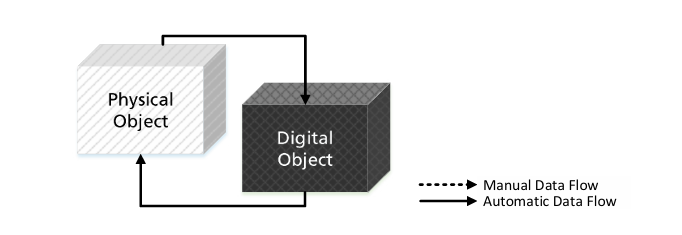
\includegraphics[width=0.75\textwidth]{figures/chapter_02/dm_ds_dt.png}}{%
    \selectedFigureBox{Kritzinger et al., data-flow classification of Digital Model, Digital Shadow, and Digital Twin}{figures/chapter_02/dm_ds_dt.png}{https://doi.org/10.1016/j.ifacol.2018.08.474}}
    \caption{Digital Model, Digital Shadow, and Digital Twin integration levels. Source: \url{https://doi.org/10.1016/j.ifacol.2018.08.474}.}
    \label{fig:2-1-digital-model-shadow-twin-placeholder}
\end{figure}

\begin{footnotesize}
\setlength{\tabcolsep}{2pt}
\begin{longtable}{@{}>{\raggedright\arraybackslash}p{0.18\textwidth}>{\raggedright\arraybackslash}p{0.25\textwidth}>{\raggedright\arraybackslash}p{0.25\textwidth}>{\raggedright\arraybackslash}p{0.20\textwidth}@{}}
\caption{Data-flow distinction between digital representations}\\
\toprule
Type & Physical-to-digital flow & Digital-to-physical flow & Typical example \\
\midrule
\endfirsthead
\toprule
Type & Physical-to-digital flow & Digital-to-physical flow & Typical example \\
\midrule
\endhead
Digital Model & Manual or offline & Manual or absent & Standalone crop simulation \\
Digital Shadow & Automatic & Manual or absent & Sensor dashboard updated from field data \\
Digital Twin & Automatic & Automatic or operationally connected & Synchronized decision/control system \\
\bottomrule
\end{longtable}
\end{footnotesize}

\section{Digital Twin architecture layers}

A Digital Twin architecture is usually layered. The physical layer contains the real process or asset. The sensing layer collects measurements. The communication layer transfers data. The data layer stores and cleans information. The modeling layer represents the system state. The simulation layer evaluates scenarios. The analytics or AI layer supports prediction and optimization. The application layer presents results to users. Finally, the feedback or control layer closes the loop through recommendations or actuator commands.

In agriculture, these layers must handle biological and environmental variability. Unlike a factory machine, a crop is a living system affected by weather, soil, pests, growth stage, and management practices. Therefore, agricultural Digital Twins require both engineering infrastructure and agronomic knowledge.

\begin{figure}[H]
    \centering
    \IfFileExists{figures/chapter_02/dt_framework.png}{%
    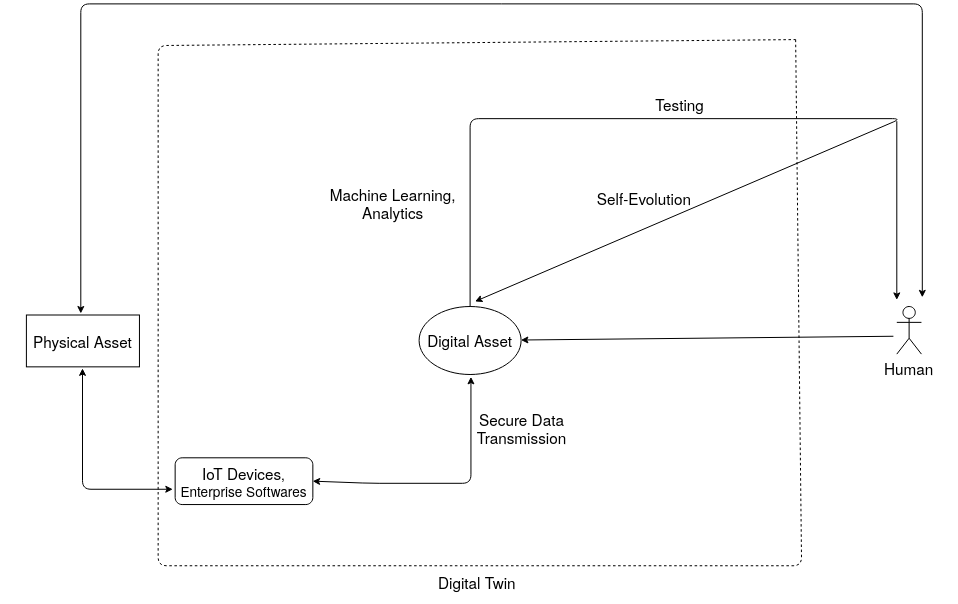
\includegraphics[width=0.75\textwidth]{figures/chapter_02/dt_framework.png}}{%
    \selectedFigureBox{Sharma et al., Figure 1, DT reference framework with components and information flows}{figures/chapter_02/dt_framework.png}{https://arxiv.org/abs/2011.02833}}
    \caption{Digital Twin reference framework with components and information flows. Source: \url{https://arxiv.org/abs/2011.02833}.}
    \label{fig:2-2-layered-digital-twin-placeholder}
\end{figure}

\section{Internet of Things as the physical-to-digital bridge}

The Internet of Things (IoT) provides the physical-to-digital connection required by smart irrigation and Digital Twins. Gubbi et al. \cite{gubbi2013iot} describe IoT as a networked environment where sensing and actuating devices blend with the physical world and share information across platforms. In agriculture, IoT devices can include soil sensors, weather stations, cameras, embedded controllers, gateways, and actuator modules.

IoT is important because a Digital Twin cannot remain synchronized without data. Sensors measure soil and environmental conditions, gateways aggregate and transmit messages, and cloud or edge services store and process them. In irrigation, IoT also supports feedback because commands can be sent to pumps and valves, while status messages can confirm execution.

\begin{footnotesize}
\setlength{\tabcolsep}{2pt}
\begin{longtable}{@{}>{\raggedright\arraybackslash}p{0.22\textwidth}>{\raggedright\arraybackslash}p{0.32\textwidth}>{\raggedright\arraybackslash}p{0.30\textwidth}@{}}
\caption{IoT functions in Digital Twin and irrigation systems}\\
\toprule
Function & Description & Example in agriculture \\
\midrule
\endfirsthead
\toprule
Function & Description & Example in agriculture \\
\midrule
\endhead
Sensing & Measuring physical variables & Soil moisture, air temperature, rainfall \\
Identification & Associating data with device, zone, or asset & Sensor ID, plot ID, timestamp \\
Communication & Sending data between devices and services & LoRa, Wi-Fi, MQTT, cellular \\
Edge processing & Cleaning or aggregating data near the field & Gateway validation, local filtering \\
Cloud/data service & Storing and exposing data for applications & Database, API, dashboard backend \\
Actuation & Applying commands to physical devices & Pump, valve, relay, fertigation unit \\
\bottomrule
\end{longtable}
\end{footnotesize}

\section{Artificial intelligence: general definition}

Artificial intelligence is a broad field concerned with building systems that perform tasks associated with perception, reasoning, learning, communication, planning, and action. The Dartmouth proposal that introduced the field framed AI around the idea that aspects of learning and intelligence could be described precisely enough for machines to simulate them \cite{mccarthy1955dartmouth}. Modern AI includes symbolic reasoning, search, probabilistic models, machine learning, deep learning, language models, and agent systems.

In agricultural decision support, AI is useful when the decision cannot be expressed only as a simple fixed rule. Irrigation depends on nonlinear relationships between weather, soil, crop, and management actions. AI methods can learn from historical data, detect patterns, classify risk, predict future states, or help users interact with complex data through natural language.

\section{Machine learning}

Machine learning (ML) is a subfield of AI in which models improve their performance by learning patterns from data. In irrigation, ML can be used for classification, regression, forecasting, anomaly detection, and optimization. Examples include predicting whether irrigation is needed, estimating future soil moisture, forecasting evapotranspiration, detecting sensor faults, or estimating irrigation duration.

Classical ML methods such as Decision Trees, Random Forests, Support Vector Machines, Gradient Boosting, and k-nearest neighbors are often suitable for tabular sensor data. Random Forests are especially common because they combine many decision trees and can model nonlinear relationships while remaining easier to train than many deep learning architectures \cite{breiman2001randomforest}.

\begin{footnotesize}
\setlength{\tabcolsep}{2pt}
\begin{longtable}{@{}>{\raggedright\arraybackslash}p{0.20\textwidth}>{\raggedright\arraybackslash}p{0.28\textwidth}>{\raggedright\arraybackslash}p{0.36\textwidth}@{}}
\caption{Machine learning tasks in irrigation and agriculture}\\
\toprule
Task & Typical model family & Example output \\
\midrule
\endfirsthead
\toprule
Task & Typical model family & Example output \\
\midrule
\endhead
Classification & Decision Tree, Random Forest, SVM & Irrigate / do not irrigate \\
Regression & Random Forest, Gradient Boosting, neural network & Predicted soil moisture or water amount \\
Time-series forecasting & ARIMA, LSTM, temporal neural network & Future moisture or evapotranspiration \\
Anomaly detection & Isolation Forest, statistical threshold & Sensor fault or abnormal reading \\
Optimization & Reinforcement learning, evolutionary algorithms & Irrigation policy or schedule \\
\bottomrule
\end{longtable}
\end{footnotesize}

\section{Deep learning}

Deep learning (DL) is a machine learning approach based on neural networks with multiple processing layers. LeCun, Bengio, and Hinton \cite{lecun2015deeplearning} explain that deep learning learns representations at multiple levels of abstraction. This makes it powerful for unstructured or high-dimensional data such as images, audio, text, and long time series.

In agriculture, deep learning is widely used for crop disease detection, weed recognition, fruit detection, yield estimation, remote sensing image analysis, and time-series prediction. In irrigation, recurrent networks, temporal convolutional networks, and LSTM models can be used to forecast soil moisture or water demand. However, deep learning usually requires larger datasets, more computation, and stronger validation than classical ML.

\begin{figure}[H]
    \centering
    \IfFileExists{figures/chapter_02/dl_backprop.jpg}{%
    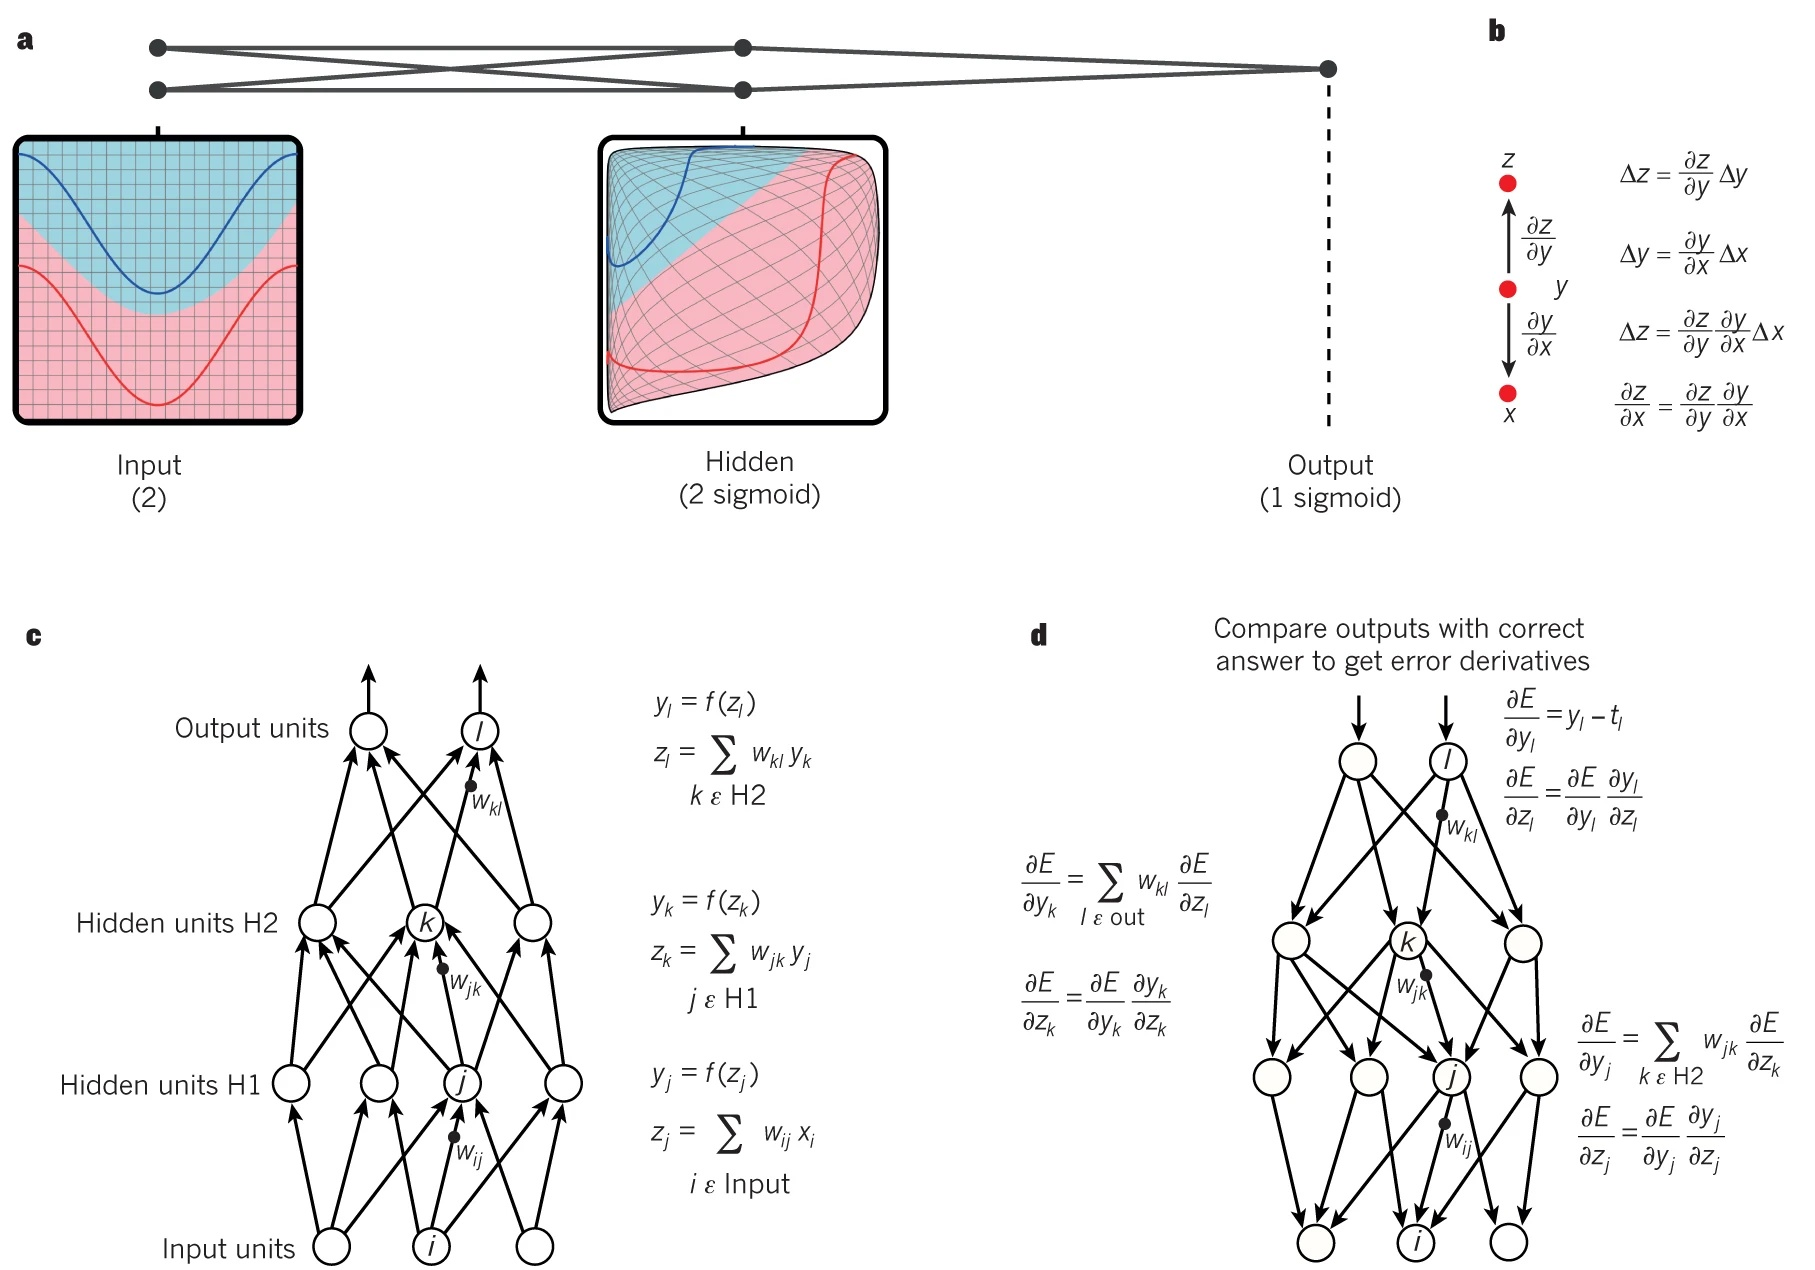
\includegraphics[width=0.75\textwidth]{figures/chapter_02/dl_backprop.jpg}}{%
    \selectedFigureBox{LeCun, Bengio, and Hinton, Nature 2015, Figure 1, ``Multilayer neural networks and backpropagation''}{figures/chapter_02/dl_backprop.jpg}{https://www.nature.com/articles/nature14539}}
    \caption{Multilayer neural networks and backpropagation. Source: \url{https://www.nature.com/articles/nature14539}.}
    \label{fig:2-3-deep-learning-placeholder}
\end{figure}

\section{Large language models}

Large language models (LLMs) are deep learning models trained on large text corpora to predict, generate, summarize, translate, and reason over language. They are part of the broader family of foundation models, which Bommasani et al. \cite{bommasani2021foundationmodels} describe as models trained at scale and adaptable to many downstream tasks. Modern LLMs are usually based on the Transformer architecture introduced by Vaswani et al. \cite{vaswani2017attention}. Brown et al. \cite{brown2020languagemodels} showed that scaling autoregressive language models can improve few-shot behavior, meaning that tasks can be specified through instructions and examples in text.

LLMs are not irrigation models by themselves. Their value in agricultural systems is mainly at the interaction and knowledge layer. They can help users query sensor histories, summarize alerts, explain model outputs, generate reports, retrieve agronomic documentation, or support natural-language interfaces. They must be used carefully because generated text can be incorrect, unsupported, or overconfident. For technical and agronomic decisions, LLM outputs should be grounded in validated data, citations, and human review.

\begin{figure}[H]
    \centering
    \IfFileExists{figures/chapter_02/transformer.png}{%
    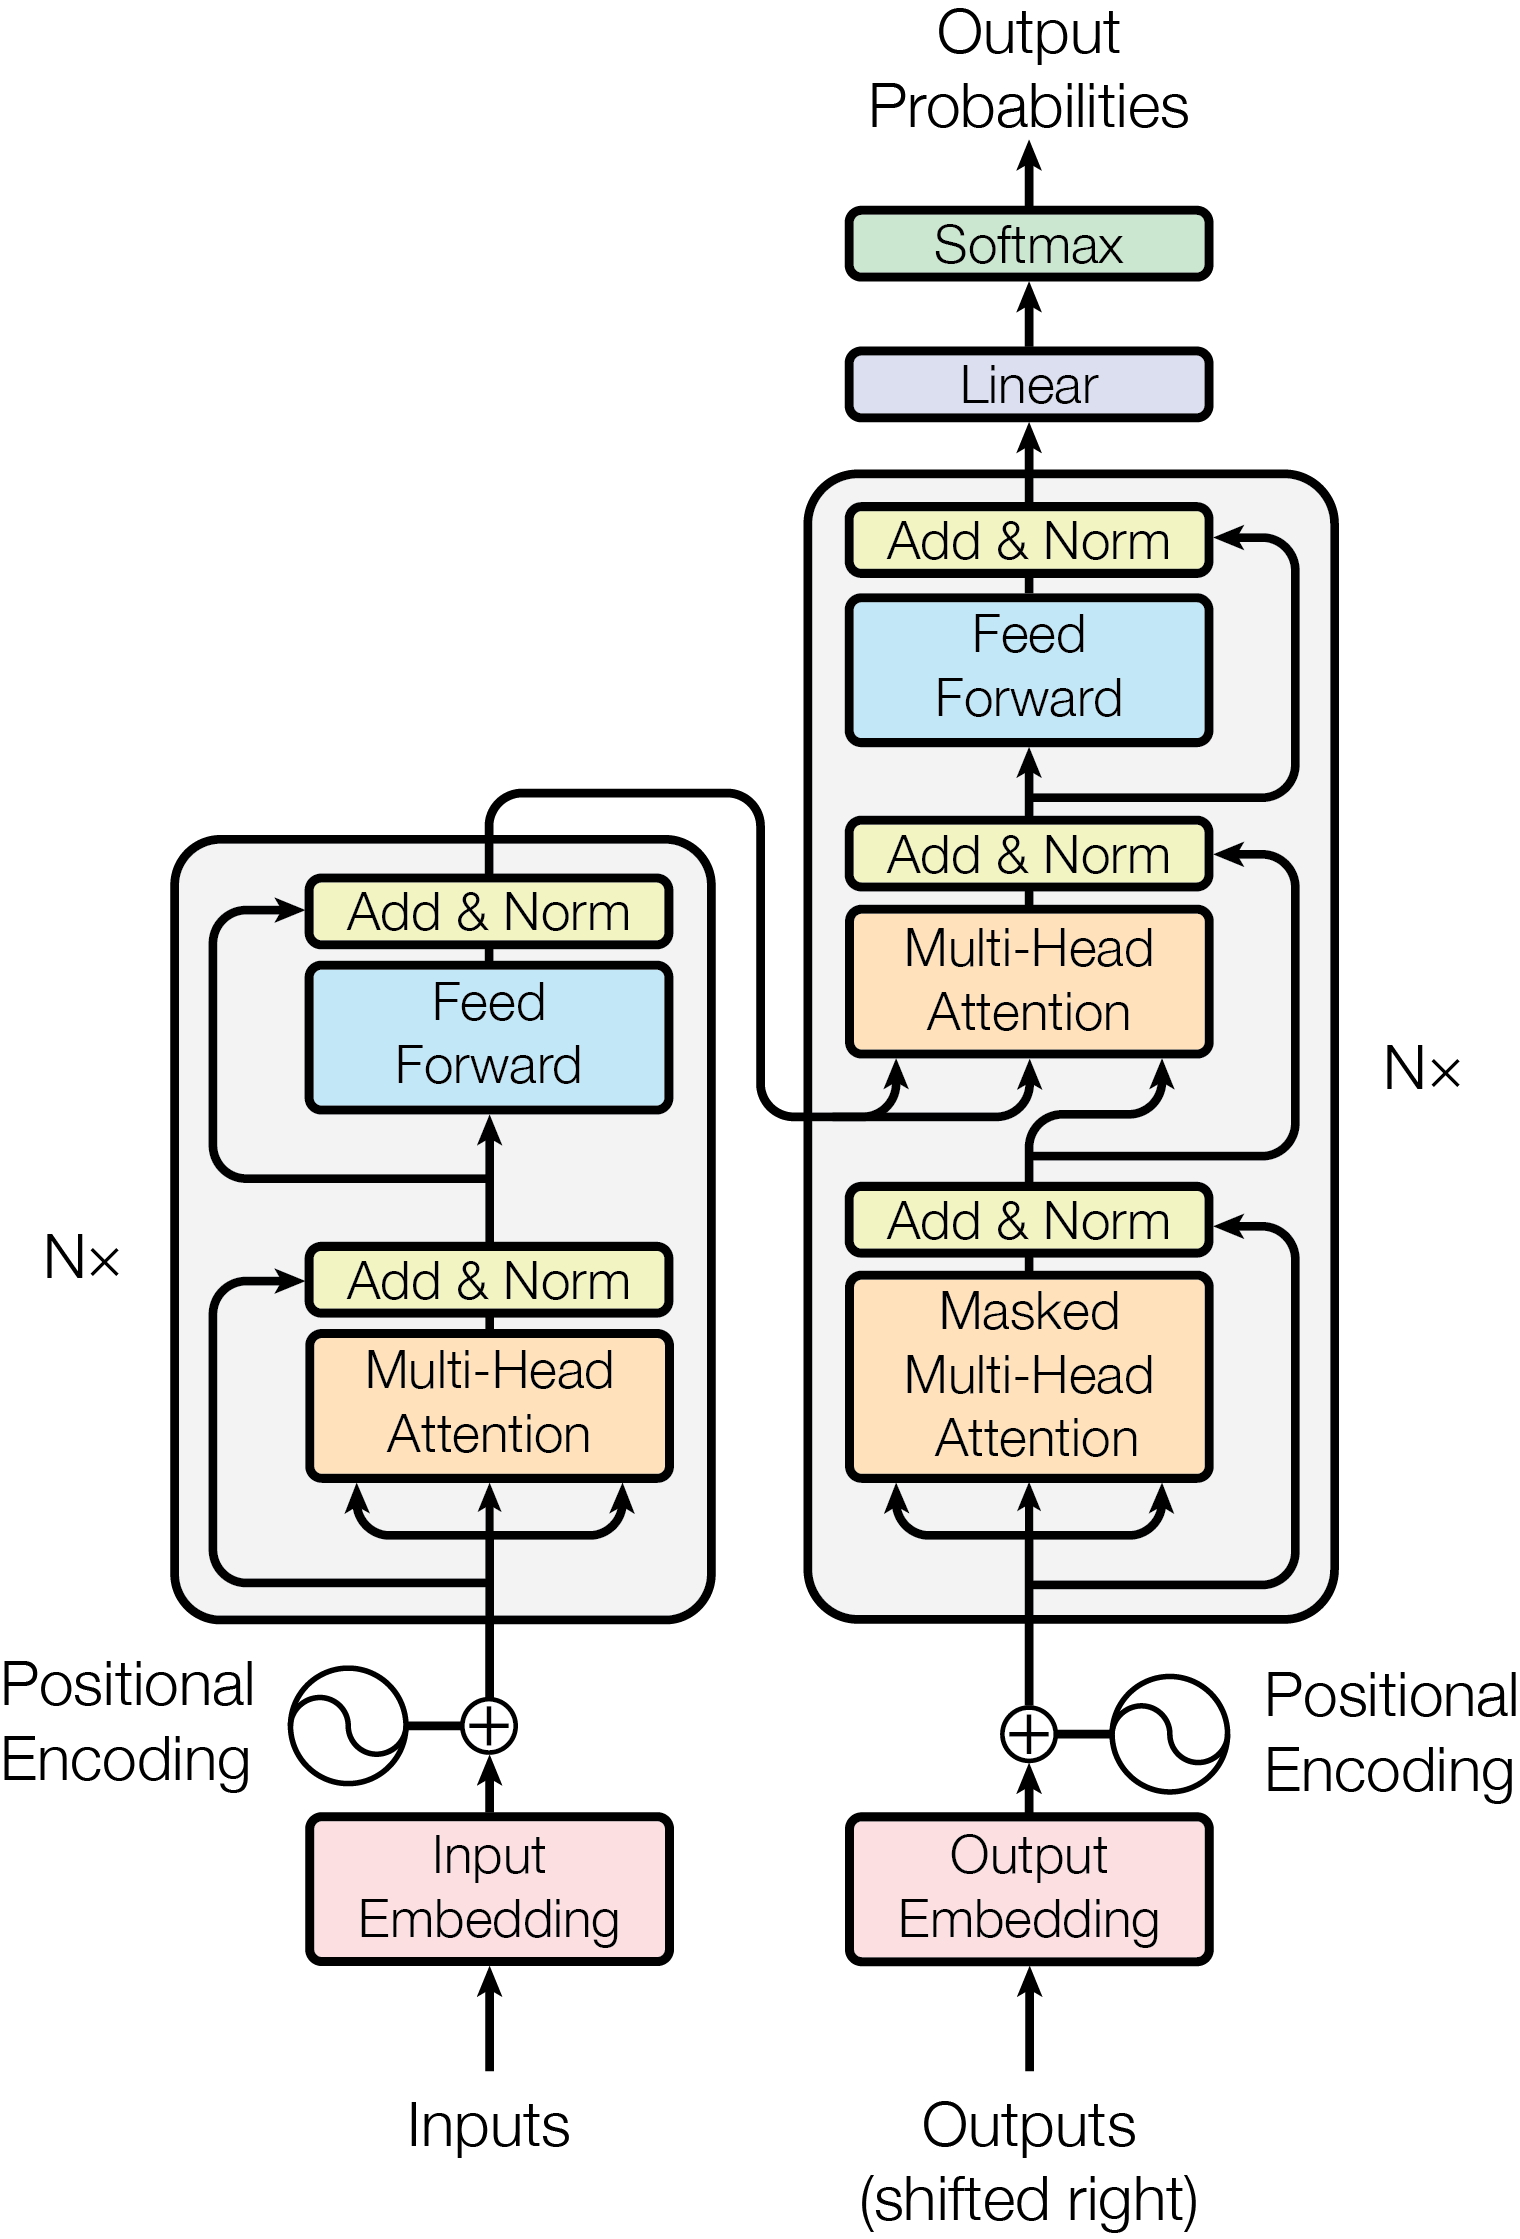
\includegraphics[width=0.55\textwidth]{figures/chapter_02/transformer.png}}{%
    \selectedFigureBox{Vaswani et al., Figure 1, ``The Transformer - model architecture''}{figures/chapter_02/transformer.png}{https://arxiv.org/abs/1706.03762}}
    \caption{The Transformer model architecture. Source: \url{https://arxiv.org/abs/1706.03762}.}
    \label{fig:2-4-transformer-placeholder}
\end{figure}

\section{Multi-agent systems}

Multi-agent systems (MAS) study systems composed of multiple interacting agents. Wooldridge and Jennings \cite{wooldridge1995intelligentagents} describe intelligent agents through properties such as autonomy, reactivity, proactiveness, and social ability. In a multi-agent system, several agents may observe, communicate, negotiate, coordinate, or act in a shared environment.

In agriculture, a multi-agent view can be useful when decisions are distributed. For example, one agent may monitor weather, another may evaluate soil state, another may optimize irrigation scheduling, and another may communicate with a human operator. In collective irrigation networks, different farms or zones may compete for limited water, making coordination and negotiation important.

Recent work also connects LLMs with agent systems. Foundation models can provide language understanding and planning capabilities, while agent frameworks organize tool use, memory, roles, and communication. However, the classical MAS literature remains important because it provides established concepts for coordination, autonomy, communication protocols, and decentralized decision-making.

\begin{footnotesize}
\setlength{\tabcolsep}{2pt}
\begin{longtable}{@{}>{\raggedright\arraybackslash}p{0.20\textwidth}>{\raggedright\arraybackslash}p{0.29\textwidth}>{\raggedright\arraybackslash}p{0.35\textwidth}@{}}
\caption{AI families and their possible roles in agricultural decision support}\\
\toprule
AI family & Main idea & Possible role in agriculture \\
\midrule
\endfirsthead
\toprule
AI family & Main idea & Possible role in agriculture \\
\midrule
\endhead
Machine learning & Learn prediction rules from structured data & Irrigation classification, soil moisture prediction \\
Deep learning & Learn representations from high-dimensional data & Image analysis, disease detection, time-series forecasting \\
Large language models & Generate and reason over natural language & Explanations, reporting, question answering, user interface \\
Multi-agent systems & Coordinate autonomous or semi-autonomous agents & Distributed monitoring, scheduling, negotiation, control \\
\bottomrule
\end{longtable}
\end{footnotesize}

\section{Human-in-the-loop decision support}

Agricultural AI and Digital Twins should not be treated as replacements for agronomic expertise. Farmers and agronomists know local practices, crop history, irrigation constraints, and risk tolerance. Human-in-the-loop decision support keeps the human user involved in interpretation, validation, and action, especially when physical actuators are involved.

This approach is particularly important for irrigation because wrong recommendations can have physical and economic consequences. A useful system should therefore provide evidence, confidence, explanations, historical context, and manual override options. Automation can increase efficiency, but trust depends on transparency, validation, and the ability to correct or reject recommendations.

\section{Challenges}

Digital Twin and AI adoption in agriculture faces several challenges. Data may be noisy, missing, poorly calibrated, or collected at different time scales. Models trained in one crop, soil type, or climate may not generalize to another. Communication networks may be unreliable in rural areas. Security and privacy are also important because connected systems can expose farm data or actuator control channels.

AI introduces additional risks: overfitting, lack of interpretability, bias in datasets, weak field validation, and excessive confidence in predictions. LLMs add the risk of unsupported generation. Multi-agent systems add coordination and safety challenges. For these reasons, background concepts must be connected to validation methods in later chapters.

\section{Conclusion}

This chapter defined Digital Twins, IoT, and artificial intelligence as enabling concepts for data-driven agricultural systems. Digital Twins provide synchronized virtual representations of physical processes. IoT provides the sensing, communication, and actuation bridge. AI provides methods for prediction, representation learning, language interaction, and distributed coordination. These foundations support the next part of the thesis, where the literature is reviewed and compared.
